% THIS IS SIGPROC-SP.TEX - VERSION 3.1
% WORKS WITH V3.2SP OF ACM_PROC_ARTICLE-SP.CLS
% APRIL 2009
%
% It is an example file showing how to use the 'acm_proc_article-sp.cls' V3.2SP
% LaTeX2e document class file for Conference Proceedings submissions.
% ----------------------------------------------------------------------------------------------------------------
% This .tex file (and associated .cls V3.2SP) *DOES NOT* produce:
%       1) The Permission Statement
%       2) The Conference (location) Info information
%       3) The Copyright Line with ACM data
%       4) Page numbering
% ---------------------------------------------------------------------------------------------------------------
% It is an example which *does* use the .bib file (from which the .bbl file
% is produced).
% REMEMBER HOWEVER: After having produced the .bbl file,
% and prior to final submission,
% you need to 'insert'  your .bbl file into your source .tex file so as to provide
% ONE 'self-contained' source file
%
% Questions regarding SIGS should be sent to
% Adrienne Griscti ---> griscti@acm.org
%
% Questions/suggestions regarding the guidelines, .tex and .cls files, etc. to
% Gerald Murray ---> murray@hq.acm.org
%
% For tracking purposes - this is V3.1SP - APRIL 2009

%\documentclass{acm_proc_article-sp}
\documentclass{sig-alternate}
\usepackage[numbers, sort, compress]{natbib}
\usepackage{graphics}
\usepackage{graphicx}
\usepackage{epstopdf}
\usepackage{color}
\usepackage{hyperref}
\usepackage{pdfsync}
\usepackage{mdwlist}

\begin{document}

\conferenceinfo{ECMLS'12,} {}
\CopyrightYear{2012}
\crdata{978-1-4503-0702-4/11/06}
\clubpenalty=10000
\widowpenalty = 10000


%\title{A Sample {\ttlit ACM} SIG Proceedings Paper in LaTeX
%Format\titlenote{(Does NOT produce the permission block, copyright information nor page numbering). For use with ACM\_PROC\_ARTICLE-SP.CLS. Supported by ACM.}}

\newif\ifdraft
\drafttrue                                                                                                   

\ifdraft
% \newcommand{\reviewer}[1]{ {\textcolor{blue}    { ***Reviewer:     #1 }}}
 \newcommand{\jkimnote}[1]{{\textcolor{green}   { ***Joohyun:   #1 }}}
 \newcommand{\jhanote}[1]{  {\textcolor{red}     { ***SJ: #1 }}}
  \newcommand{\pmnote}[1]{  {\textcolor{red}     { ***Pradeep: #1 }}}
 \newcommand{\todo}[1]{  {\textcolor{red}     { ***TODO: #1 }}}
 \newcommand{\fix}[1]{  {\textcolor{red}     { ***FIX: #1 }}}
 \newcommand{\ny}[1]{  {\textcolor{red}     { ***NY: #1 }}}
 \newcommand{\reviewer}[1]{}
\else
 \newcommand{\reviewer}[1]{}
 \newcommand{\jkimnote}[1]{}
 \newcommand{\pmnote}[1]{}
 \newcommand{\jhanote}[1]{}
 \newcommand{\todo}[1]{  {\textcolor{red}     { ***TODO: #1 }}}
 \newcommand{\fix}[1]{}                                                                                     
\fi

\title{Understanding MapReduce-based Next-Generation Sequencing
  Alignment on Distributed Cyberinfrastructure}

%\title{Next-Generation Sequencing Reads Alignment Using Pilot-based SAGA-MapReduce}

\numberofauthors{3} %  in this sample file, there are a *total*
% of EIGHT authors. SIX appear on the 'first-page' (for formatting
% reasons) and the remaining two appear in the \additionalauthors section.
%
\author{
% You can go ahead and credit any number of authors here,
% e.g. one 'row of three' or two rows (consisting of one row of three
% and a second row of one, two or three).
%
% The command \alignauthor (no curly braces needed) should
% precede each author name, affiliation/snail-mail address and
% e-mail address. Additionally, tag each line of
% affiliation/address with \affaddr, and tag the
% e-mail address with \email.
%
\alignauthor Pradeep Kumar Mantha\\
       \affaddr{Center for Computation and Technology}\\
       \affaddr{Louisiana State University}\\
       \affaddr{216 Johnston}\\
       \affaddr{Baton Rouge, LA}
       \email{pradeepm66@gmail.com}
\alignauthor Andre Luckow\\
       \affaddr{Center for Computation and Technology}\\
       \affaddr{Louisiana State University}\\
       \affaddr{216 Johnston}\\
       \affaddr{Baton Rouge, LA}
\alignauthor Nayong Kim\\
       \affaddr{Center for Computation and Technology}\\
       \affaddr{Louisiana State University}\\
       \affaddr{216 Johnston}\\
       \affaddr{Baton Rouge, LA}
\and
\alignauthor Joohyun Kim\titlenote{Author for correspondence}\\
       \affaddr{Center for Computation and Technology}\\
       \affaddr{Louisiana State University}\\
       \affaddr{216 Johnston}\\
       \affaddr{Baton Rouge, LA} \\
       \email{jhkim@cct.lsu.edu}
\alignauthor Shantenu Jha\titlenote{Author for correspondence}\\
      \affaddr{Center for Computation and Technology}\\
     \affaddr{Louisiana State University}\\
      \affaddr{214 Johnston}\\
      \affaddr{Baton Rouge, LA}
     \email{sjha@cct.lsu.edu}
}
% There's nothing stopping you putting the seventh, eighth, etc.
% author on the opening page (as the 'third row') but we ask,
% for aesthetic reasons that you place these 'additional authors'
% in the \additional authors block, viz.
%\additionalauthors{Additional authors: John Smith (The Th{\o}rv{\"a}ld Group,
%email: {\texttt{jsmith@affiliation.org}}) and Julius P.~Kumquat
%(The Kumquat Consortium, email: {\texttt{jpkumquat@consortium.net}}).}
\date{25 Feb. 2012}
% Just remember to make sure that the TOTAL number of authors
% is the number that will appear on the first page PLUS the
% number that will appear in the \additionalauthors section.

\maketitle
\begin{abstract} 
  Although localization of Next-Generation Sequencing data is suitable
  for many analysis and usage scenarios, it is not universally
  desirable nor possible. However most solutions ``impose'' the
  localisation of data as a pre-condition for NGS analytics.  We
  analyze several existing tools and technqiues that use MapReduce
  programming model for Next-Generation Sequencing (NGS) data analysis
  to determine their effectiveness and extensibilty to support
  distributed data scenarios. We find limitations at multiple
  levels. To overcome these limitations, we developed a Pilot-based
  MapReduce (PMR) -- which is a novel implementation of MapReduce
  using a Pilot task and data management implementation.  PMR provides
  an effective means by which a variety of new or existing methods for
  NGS and downstream analysis can be carried out whilst providing
  efficiency and scalability across multiple clusters.  We compare and
  contrast the PMR approach to similar capabilities of SEQAL and
  Crossbow, two other tools which are based on conventional
  Hadoop-based MapReduce for NGS reads alignment and duplicate removal
  or SNP finding, respectively. We find that a PMR is a viable tool to
  support distributed NGS analytics, as well as providing a framework
  that support task-level concurrency for a wide range of NGS data
  analysis and downstream processing.
\end{abstract}

% We analyze several existing tools and technqiues that use MapReduce
% programming model for Next-Generatiion Sequencing (NGS) data analysis.
% Our approach is based on the Pilot-based SAGA-MapReduce (PMR)
% framework which extends previously introduced SAGA-MapReduce with a
% Pilot task and data management implementation.  PMR provides an
% effective means to develop software tools with which a variety of
% existing or novel methods for NGS data and downstream analysis are
% carried out and more importantly achieve scalability across multiple
% clusters.  As demonstrating examples for the capabilities of our
% PMR-based approach, we implemented similar capabilities of SEQAL and
% Crossbow, two other tools which are based on conventional Hadoop-based
% MapReduce for NGS reads alignment and duplicate removal or SNP
% finding, respectively.  The comparison to these tools allows us to
% characterize our approach with PMR as a viable tool for the
% scale-across requirement as well as a versatile parallelism framework
% for a wide range of NGS data analysis and process tools.  The
% scalability with distributed sequencing data and the potentials for
% other analysis applications are discussed.


\category{D.1.3}{Software}{Concurrent Programming}{ Distributed
  programming/parallel programming} \category{J.3}{Computer
  Applications}{Bioinformatics, Mapping}


% A category with the (minimum) three required fields
%\category{H.4}{Information Systems Applications}{Miscellaneous} %Acategory including the fourth, optional field follows...
%\category{D.2.8}{Software Engineering}{Metrics}[complexity measures,performance measures]

\terms{Design, Experimentation, Performance}

 \keywords{Genome Sequence Alignment, BWA, Human Genome, RNA-Seq Data,
  MapReduce, Distributed Computing, Simple API for Grid
  Applications (SAGA), Pilot Job and Data}

%\keywords{ACM proceedings, \LaTeX, text tagging} % NOT required for Proceedings 
%\keywords{RNA conformation energy landscape, Runtime Environment, SAM-I riboswitch,
% S gene of Bovine Corona Viral Genome} % NOT required for Proceedings

\section{INTRODUCTION} 
Recent advances in high-throughput DNA sequencing technologies such as Next-Generation Sequencing (NGS) platforms have imposed unprecedented challenges in areas of bioinformatics, computational biology, and biocomputing in general\cite{metzker2010,1000genome,wang2009-natrevgen,alex2009,mcpherson2009}.  With astronomically explosive volumes of raw data and processed data, along with required computational tasks that often need scalable infrastructure, these challenges are to some extent novel because of the need of an integrative solution leveraging algorithmic advances, computational implementations exploiting modern parallel processor or cluster architectures, and infrastructure developments altogether. Indeed, still at this moment it is not uncommon to find many biologists who have sequencing data sets in their hand and want to pursue their biological/biomedical queries in a timely fashion but are puzzled by so-many-tools with different algorithms and computational requirements including the installation, maintenance, and update of the software tools. 

Among many directions for overcoming such challenges, the use of parallelism for distributed data is an emerging strategy and in fact the programming model of MapReduce along with Cloud environments has been widely touted as an efficient solution for big data problems\cite{mapreduce-2004-dean,schatz-nature-biotech-2010, taylor2010}.  Several tools using MapReduce were already introduced for NGS data analysis such as read alignment onto a reference genome\cite{cloudburst, gatk,langmead2009,seal2011,langmead2010, taylor2010}.

In this work, we present the development of a Next-Generation Sequencing reads alignment tool using Pilot-based SAGA-MapReduce (PMR) which is a recent re-implementation of SAGA-MapReduce with a newly developed Pilot-based approach\cite{Sehgal2011590,pmr2012}.  Indeed, PMR provides a viable solution for computational challenges with NGS data analytics, in particular, arising from the required scalability for dealing with ever-growing data volume, variety, and demand for time-to-solution as well as an effective software development for a diverse and ever-increasing software tools, in particular the emergence of revolutionary NGS techniques such as RNA-Seq.  Our implementation of the MapReduce programming model supports the development of dynamic applications which represent applications executed in distributed resources across the boundary of a cluster system or the mix of HPC grids and Clouds via effective and dynamic task and data management.  This aspect is particularly contrasted to other approaches using Hadoop-based MapReduce implementations \cite{cloudburst,langmead2009,seal2011,langmead2010}.  

To demonstrate the capabilities with PMR, we primarily attempt the comparative experiments to the two known MapReduce-based tools, SEQAL in the SEAL package and Crossbow\cite{seal2011,lanmead2010}.  The two tools were developed for carrying out two different analyses; the alignment step was implemented as the first step with BWA and Bowtie, respectively but the second analysis is duplicate read removal for SEQAL whereas SNP finding for Crossbow.  This comparison provides clear evidence for promising features with PMR for NGS data analysis tools combining the read alignment and successive tasks.  Those features include i) scalability across multiple heterogeneous infrastructures ii) framework supporting a quick turnaround of development cycles and extensions iii) effectiveness for a big data problem with distributed data, implying that distributed cyberinfrastructure would be another viable compute and data management environment for high-throughput DNA sequencing data.  

Before we present the contribution and outline of the paper, we
clarify our usage of the different types of scaling that this paper
will be concerned with: {\it scale-up} -- or the most common type of
scaling behavior, is a reference to the ability (performance) of using
many cores efficiently; {\it scale-out} is a measure of the number of
tasks that can be concurrently executed \& managed; {\it scale-across}
is a measure of the number of distinct compute resources that an
application can utilize.

\pmnote{
Doesn't  scale-up and scale-out mean same thing as per above description??
In Fig 3,  as the number of nodes or cores increase, the runtime decreases- so its scales-up well.
The concurrency of tasks, increase with number of cores.. Figure -3 again shows that.
I mean both are related to the number of workers used.
}

\jhanote{Say something about tooling, something about integrated the concurrency also increased. and
  extensible environment}

\jhanote{`Unfortunately, users cannot directly deploy a MapReduce
  framework such as Hadoop on top of these clusters to form a single
  larger MapReduce cluster. Typically the internal nodes of a cluster
  are not directly reachable from outside. However, MapReduce requires
  the master node to directly communicate with any slave node, which
  is also one of the reasons why MapReduce frameworks are usually
  deployed within a single cluster. Therefore, one challenge is to
  make multiple clusters act collaboratively as one so it can more
  efficiently run MapReduce.''}

\pmnote{Why do we need a distributed mapreduce framework to process
  distributed data on multiple frameworks?  1. To process the data on
  a single cluster takes more time and getting shared HPC resources to
  process that huge is also difficult. So distributing the data( Which
  can be a one time setup) to multiple clusters allows the flexibility
  to use more computation and process the data quickly.  2. "Although
  commercial clouds can provide virtually unlimited computation and
  storage resources on-demand, due to financial, security and possibly
  other concerns, many researchers still run experiments on a number
  of small clusters with limited number of nodes that cannot unleash
  the full power of MapReduce." - {Hierarchical mapreduce} }

The paper is organized as follows. In the following Section~\ref{sec:materials_and_methods}, the data sets we used for this work and experimental methods are presented.   In Section~\ref{sec:experiments}, we describe the rational and experimental details for this paper.  After that, in Section~\ref{sec:results}, results for parallel performance measurements and comparison of our results with SEQAL and Crossbow which represents applications that use the open source Hadoop-based MapReduce\cite{hadoop-url, taylor2010,seal_2011_mapred,seal2011} are presented.  Finally, in Section~\ref{sec:discussions}, we will give discussions and conclude this paper with remarks focusing on implications of our experiments for development of biological information infrastructure around NGS data for a short term goal of RNA-Seq data analysis and for a long term goal for an integrative research infrastructure that provides various holistic services of downstream analyses streamlined with effective computation of NGS data and analytics.



\section{Materials and Methods}\label{sec:materials_and_methods}
\subsection{NGS Data Sets and Target Analyses}
\subsubsection{Data Sets}

For this work, we used the paired-end sequence RNA-Seq data from the Flemington lab, which had originated from a Human Burkitt's lymphoma cell line\cite{erik_2010}.  The read length is 100 for both directions of paired-end data, and the total size of each data set is about 20.1 GB containing 70927422 reads.  For the experiments that use a varying size of sequencing data, we simply take the required amount of reads by partitioning the entire data.  The file format of sequencing data is fasta and all manipulation of sequencing data was conducted by in-house python scripts and freely available tools such as samtools\cite{samtools}.  

\subsubsection{DNA Sequence Alignment}

The short reads alignment and the de-novo assembly are the required first steps in every pipeline software tool aiming biological discovery with sequencing data from NGS platforms.  Considering the fact that the de-novo assembly remains still challenging at this moment primarily arising from the complications with the short length of sequencing reads from NGS machines, in a practical sense, alignment or mapping is taken as the first task in most of cases.  In fact, for RNA-Seq data analysis, in particular with eukaryote genomes, the spliced aligner such as TopHat\cite{pepke2009} is needed. In this work, we consider the alternative strategy such that the non-spliced aligner is used and later splicing events are detected separately, justifying the use of non-spliced aligners such as BWA and Bowtie for the RNA-Seq data.  The reference genome used with these aligners is hg19.

\subsubsection{Other Data Analyses}

After alignment of sequenced reads onto the reference genome, a duplicate read removal step might be required because sample preparation processes before sequencing might contain artifacts stemming from high-throughtput read amplification; many duplicates introduced are not relevant to true biological conditions.  For characterizing our framework, we compare our results with the SEQAL tool of SEAL package since SEQAL aims to carry out the read alignment and duplicate removal.  SEQAL uses BWA for the alignment and for the duplicate removal, implements the same criteria as the Picard MarkDuplicates command\cite{seal2011,seal_2011_mapred}.  On the other hand, information about aligned reads are essential for many downstream analyses such as genome variation study, transcriptome analysis, and other various complex functional genomics and pathway analysis.  For example, Crossbow, the tool we investigated by the comparative experiments, aims to SNP finding along with aligned results\cite{langmead2009}.  Interestingly, Crossbow use the aligner, Bowtie, and thus our PMR-based tool is extended to implement Bowtie, in addition to BWA for the comparison with Crossbow.  Note that Bowtie is well-known for its efficiency in memory requirement and computation, but the current version doe not support gapped alignment whereas BWA does.

\subsection{Experimental Set-up for NGS Read Alignment and Duplicate Removal}
\subsubsection{HPC Resources}
For this work, we used two Futuregrid systems, SIERRA and HOTEL.  More details on the specification of these machines can be found from the web page of Futuregrid\cite{futuregrid_url}.  In brief, two systems are multi-node clusters and equipped with the PBS job scheduler and Hadoop, implying that the systems are appropriate to test our PMR and to compare our results with Hadoop-based tools.

\subsubsection{MapReduce-based NGS Data Analytics using Pilot-based SAGA-MapReduce (PMR)}
The two combined steps such as alignment and duplicate removal or alignment and SNP finding are attractive targets for  parallelizing tasks by using MapReduce; the read alignment step is conducted as a Map phase and duplicate removal or SNP finding as a Reduce phase.  Note that a certain kind of combination for designing a MapReduce-based tool is immediately conceivable for other advanced downstream analyses such as transcript quantification or peak calling for other advanced NGS protocols.  The development for such tools will be announced in the future works.

The schematic workflow and architecture for running PMR is presented in Fig.~\ref{fig:arch-pj-saga-mr}.  As indicated, we need to configure computational tasks of the map phase and the reduce phase including the number of workers, available fine-grained parallelism options of software tools used for each phase, and configurations for Pilot Job (BigJob).  Note that we can choose many different combinations of these configurations (i.e. associated with parallel options with used software tools, and Pilot and MapReduce levels) for different strategies that tune the parallelism for a target analysis (in which map and reduce phases are decoupled, of course) differently by carefully considering fine-grained and coarse-grained parallelism levels.    

\begin{center}
\begin{table*}[ht]
{\small
\hfill{}
\begin{tabular}{|l|l|c|c|c|c|c|c|}
\hline
  & \textbf{P-SAGA-MR}\cite{pmr2012} & \textbf{SEQAL}\cite{seal2011} & \textbf{Crossbow}\cite{langmead2009} & \textbf{CloudBurst}\cite{cloudburst} & \textbf{GATK}\cite{gatk} \\ \hline
%\cline{3-9}
 \hline 
Key Parallelism   & Pilot-based   &  Hadoop-based/  &  Hadoop   & Hadoop-based & MR-based Structured \\ 
Stretegy  & Distributed MR & MR  & Streaming  & MR & Programming  \\
& & (Pydoop) &  & & Framework  \\ \hline
  
Hadoop & No & Yes & Yes\footnote[1] & Yes & No \\ 
Requirement  & & & &  &\\ \hline  
    
Multiple  Cluster & Yes  & Limited   & Limited  & Limited  & Limited \\
Support &  & by Hadoop &  by Hadoop & by Hadoop  & by JVM   \\ \hline

Multiple Node & Support & Not allowed  & Not allowed  & Not allowed & Not  \\
Task Supprt &  & by Hadoop & by Hadoop & by Hadoop & Easy  \\ \hline
Distributed Job and  & Advert Service  & Hadoop/HDFS & Hadoop/HDFS & Hadoop/HDFS & Java \\ 
Data Coordination &(SAGA) &  & & & Framework\\ \hline


Primary Aligner &  BWA, Bowtie,  &  BWA & Bowtie & RMAP &  BWA \\
& and Others (coming) &  &  &  &  \\ \hline
Multiple Aligner  & Straightforward & Not Straight- & Possible & Not Straight-  & Straight-  \\ 
Support &  & forward &   & forward  & forward \\\hline
Primary Tasks & Alignment/Duplicate  & Alignment/ & Alignment/ & Alignment &Various\\
  &  Removal & Duplicate & SNP Discovery & & NGS Data  \\  
           & (and Extensible &  Removal & &  & \& Downstream  \\
           & for RNA-Seq) & & &  & Analysis \\ \hline  
Extensibility for   &  High  & Medium &  Low & Low & High      \\
Multiple Tools  &      &  &  &  &   \\ \hline

\hline
\end{tabular}}
\hfill{}
\caption{Feature comparison of PMR with other tools for Next-Generation Sequencing (NGS) data analysis that primarily provides parallelism using the MapReduce framework.  $^{1}${The feature of Crossbow that can run with a desktop environment without Hadoop is not considered in the scope of this work due to the lack of scalability support.} }
 \label{table:mr-comparison}
\end{table*}
\end{center}

\subsubsection{Comparative Experiments with two Hadoop-based tools, SEQAL and Crossbow}
Among the software tools compared in ~\ref{table:mr-comparison}, we chose SEQAL of the SEAL package and Crossbow for the comparison.  Note that these two tools along with other tools such as Cloudburst and GATK are different from each other with respect to the usage mode of MapReduce and the design strategies behind each tool for parallelism, in particular, aiming NGS data processing and management as summarized in Table~\ref{table:mr-comparison}.  Importantly, SEQAL and Crossbow are Hadoop-based tools but differ in that the former is designed conventionally with implementing Map and Reduce functions whereas the latter uses Hadoop-streaming.  In the case of Crossbow, the overall analysis is taken with 4 steps.  Each step is an independent Hadoop-streaming task.  The first step is for pre-processing and the last one is for post-processing. The second one is for the alignment and the third one is for SNP finding, which uses slightly modified Bowtie and SOAPsnp.  

For the two applications, SEQAL and Crossbow, Hadoop version 0.20.2 was used with the two FutureGrid machines.  For SEQAL experiment, SEAL version 0.2.3 was used and for Crossbow experiments, we used version 1.1.2 that contains bowtie version 0.12.7 and soapsnp version 1.02.  If not specified, all options for aligners and external tools as well as SEQAL and Crossbow setting are default as suggested.  For example, BWA with SEQAL does not use the multi-threading option, whereas Crossbow sets up the default option for Bowtie with multi-threading option, "--mm" to support running many concurrent Bowtie processes on the same computer to share the memory index to avoid memory overhead effectively. Therefore, it is limited to launch a specific number of parallel search threads for increasing alignment throughput on using of Crossbow. 

The input file format for SEQAL is prq format.  SEAL, a software tool containing SEQAL as a part, has a file conversion capacity between qseq/fastq and prq format.  For SEQAL experiment, the replication factor for Hadoop configuration is set  to 1.  

In the case of Hadoop-based MapReduce tools, the needed configuration should set the number of workers per a node ($N_{W-n}$), the number of mappers ($N_M$) and the number of reducers ($N_R$) via Hadoop configuration or tool configuration.  These number should be carefully chosen along with the resource size, i.e., the number of nodes ($N_{node}$) and the number of cores in a node ($N_{cpu-n}$).  For example, the memory size of a node wold limit a possible choice for $N_{W-n}$ since such multiple workers in a node might need more memories than the total memory of the node and consequently fail to run.  Importantly, note that such parameters dictate the parallelism of a target task with MapReduce configuration as well as fine-grained parallelism that might be implemented in tasks for Map or Reduce phases.  For the input data partitioning, which is related to the number of tasks (i.e.$N_M$ or $N_R$), the chunk size used is 128MB, which is default block size and corresponding to nearly 292,763 reads. 
%
%The configuration , we set the number of nodes as 4, and the maximum map and reduce tasks is set to be 2.  We found that if the number of tasks is set to be more than 2, the issue with memory size occurred.  \pmnote{refer to reference paper}  Thus, total 8 workers were used.

PMR set-up is as follows.  Similar to the Hadoop-based MapReduce tools, the configuration requires to set $N_{node}$, $N_{cpu-n}$, $N_W$, and the size of BigJobs.  Note that $N_W$ has no limitation with the size of a node since multiple-node worker is possible when a tool executed by a work supports multi-node parallel implementation such as MPI.  Thus, with PMR, we set $N_W$, instead $N_{W-n}$.  Also, multiple clusters can be used for MapReduce. For example, the half of workers are assigned with HOTEL and the other half in SIERRA.  For a single system set up, like the two Hadoop-based MapReduce tools, all workers are now running in the system.  

Data management is an important component for any tools processing distributed data with parallel strategies and the efficiency of data transfer should be considered when a MapReduce-based tool is assessed.  Whereas Hadoop-based approaches relies upon HDFS and TCP/IP-based communication between data nodes, PMR uses SAGA Advert coordination among workers via Pilot framework (see Fig.~\ref{fig:arch-pj-saga-mr}).  PMR, indeed, is flexible and extensible for scaling across multiple clusters without the global file system support.  
 
%   \pmnote{chunksize = number of lines of fastq file ( number of sequences (292763 * 4 ) since in fastq each sequence is of 4 lines..
%tts = max( map on sierra, map on hotel)+max( time tansfer from sierra to hotel, time transfer from hotel to sierra)+max(reduce on sierra, reduce on hotel)..
%Graph : x axis- (2,4,8 input sizes) with chunk size 292763 sequences, number of workers=8, reduces=8.
%experiments repeated thrice.. }
 
For the experiments with PMR using distributed resources, we assume that all input and required data are stored initially on a single cluster to process and measure the time for distributing data.  


\section{Rational and Experiments}\label{sec:experiments}

\jhanote{need to explain which/what expeirments, how we perform them,
  and why?}

\jhanote{Motivation: distributed data requirements; MR-based sequncing
  applications comparision; challenges of the former in the latter}

Since the paper about the MapReduce programming model from Google in 2004\cite{mapreduce-2004-dean} and the emergence of Hadoop, the model has drawn significant attention from various application domains as a general strategy for parallelization of processing a large data.  In recent years, the computational biology community, in particular focusing on data analytics and downstream analyses of high-throughput deep sequencing techniques such as Next-Generation Sequencing has found the potential of MapReduce-based approaches for dealing with unprecedented data produced from the novel platforms\cite{schatz-nature-biotech-2010}.  Not surprisingly, most of software tools using MapReduce for NGS data were developed with Hadoop environment and consequently with Cloud computing environment such as Amazon EC2.  Unlike such tools, our approach with MapReduce is highlighted with Pilot-based and scalability across multiple distributed infrastructure including HPC grids and Clouds.  

For this work, our primary goal is to develop a PMR-based tool that is capable of tasks combining the alignment and various downstream analysis for genome structure studies, genotyping, transcriptome analysis, DNA-protein interaction, and sequencing data process such as duplicate read removal.  To address many interesting aspects and features, our experiments primarily target the comparison of our PMR-based approach with two other Hadoop-based approaches, SEQAL (tool for alignment and duplicate removal) and Crossbow (tool for alignment and SNP finding) that use slightly different Hadoop-based approaches.(see Table~\ref{table:mr-comparison}).  

We aim the comparative experiments with SEQAL and Crossbow with the following points.
\begin{itemize}
\item Pros and cons of Hadoop-based approaches
\item Importance of the support of scale-across 
\item Distributed data scenario for NGS data analysis and PMR's potential as a viable solution
\item Simple and straightforward parallel execution to combine fine-grained and coarse-grained parallel strategies with PMR 
\item Importance of extensibility for multiple tool supports
\item Benefit of a low development cost for extensions of capabilities 
\end{itemize}





\section{Results}\label{sec:results}

\subsection{PMR for NGS data analysis: Implementation}
In Fig.~\ref{fig:arch-pj-saga-mr}, the overall architecture of PMR is shown.  In brief, the target tasks are carried out with this order by implementing MapReduce with the Pilot framework\cite{pmr2012}. 1.PMR launches Map tasks on N clusters using the Pilot framework. 2. After the Map stage, PMR exchanges Intermediate data between clusters using Pilot-Data of Pilot framework  3. Finally, PMR launches Reduce tasks on N clusters using Pilot framework.


\begin{figure}
 \centering
%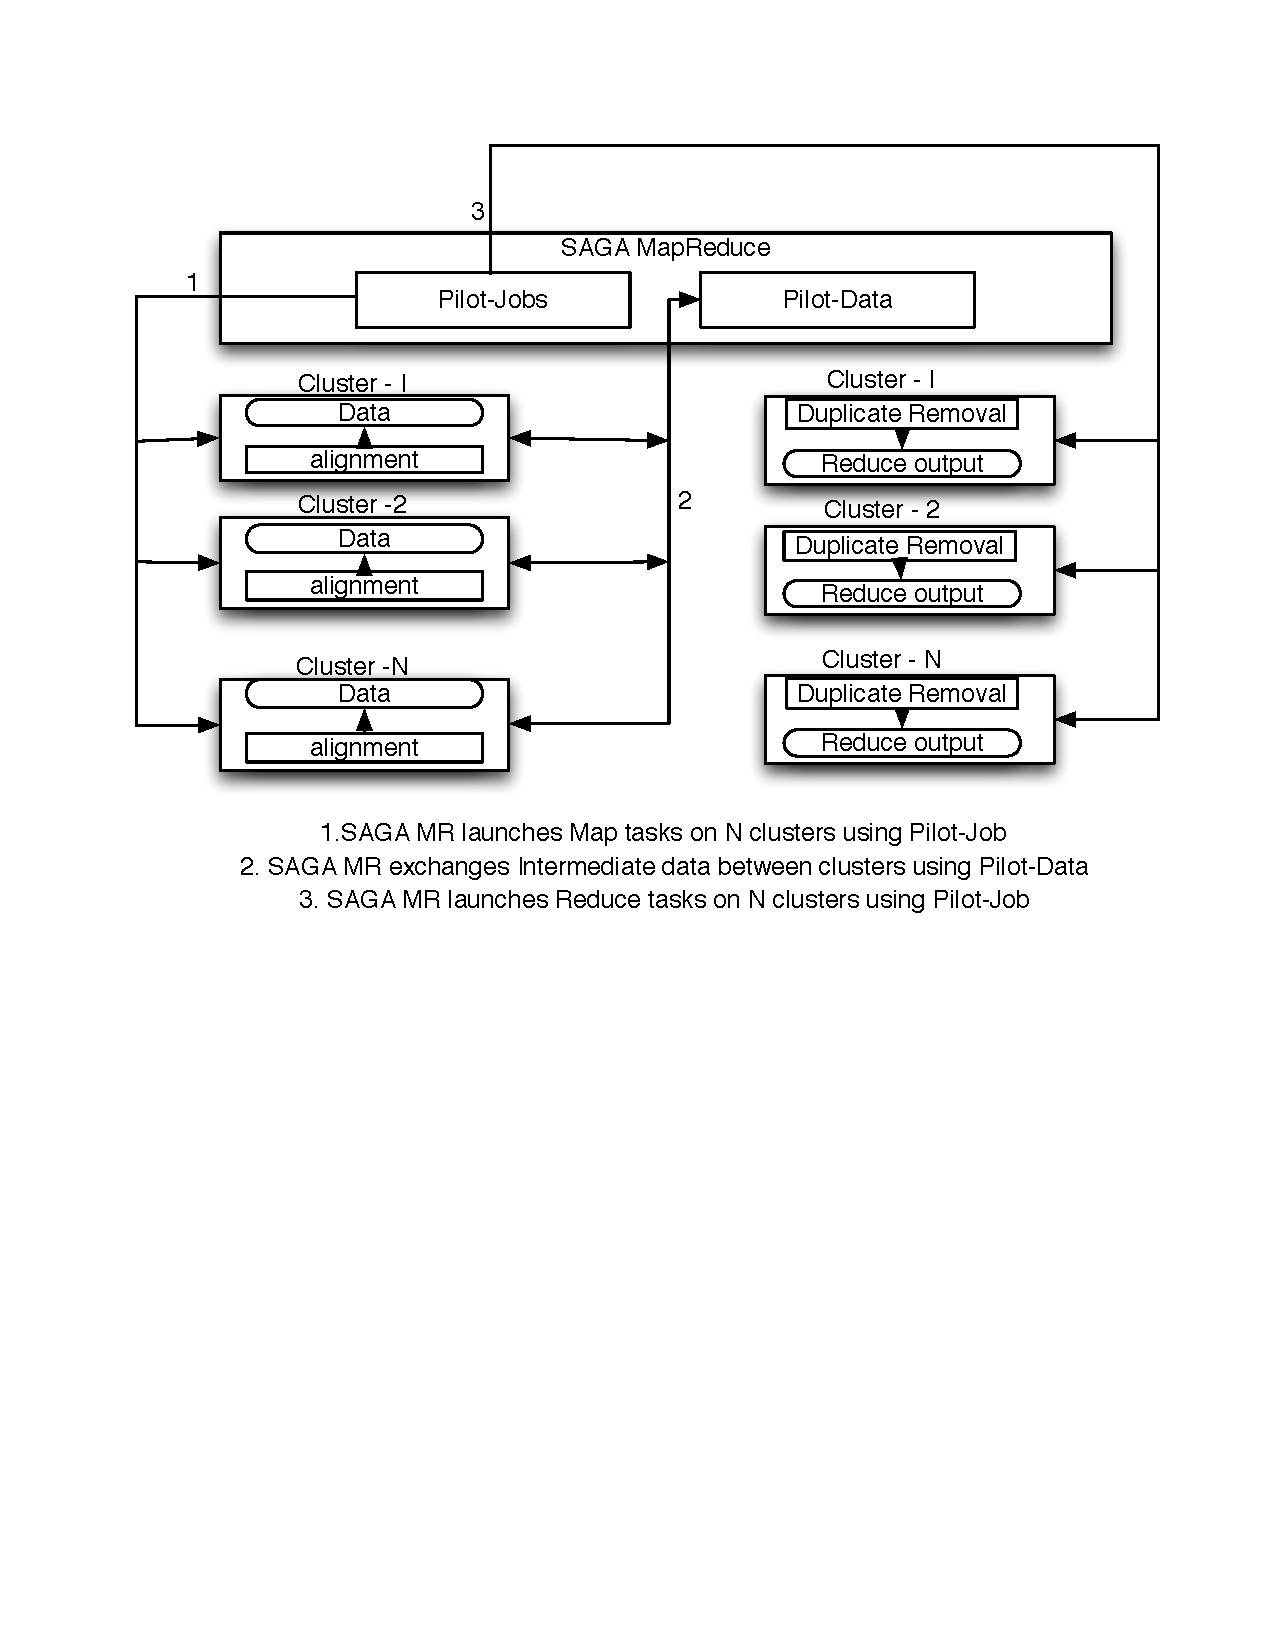
\includegraphics[scale=0.45]{figures/align-dup.pdf} 
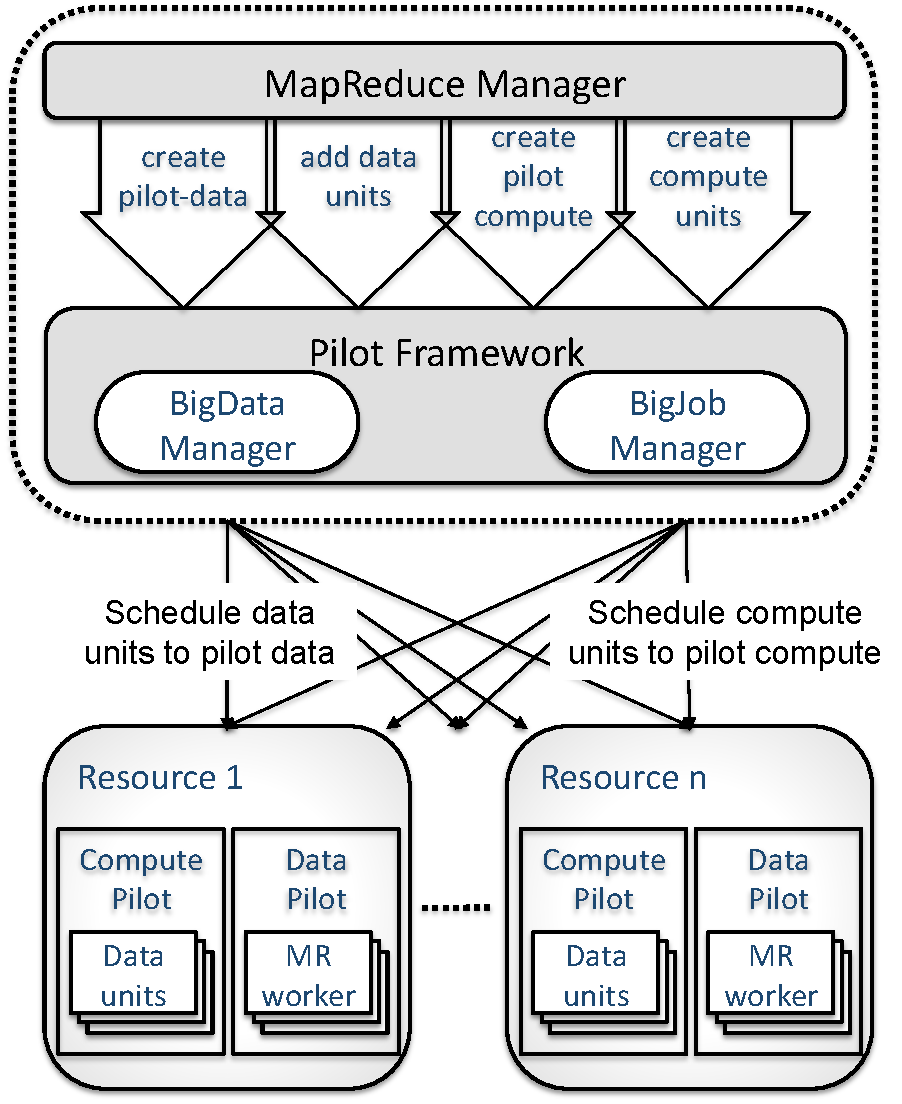
\includegraphics[scale=0.45]{figures/F1.pdf} 
\caption{\small PMR architecture and workflow for a MapReduce task}
  \label{fig:arch-pj-saga-mr} 
\end{figure}


\subsection{PMR for NGS data analysis : Reads Alignment and Duplicate Removal}

There are unique features that differentiate our approach from others, which could be beneficial for developing cyberinfrastructure for NGS data analytics and downstream analysis.  
\begin{enumerate}

\item Pilot-based MapReduce for Parallel/Concurrency framework 
\item No need of Hadoop infrastructure
\item Scalability by utilizing multiple compute resources
\item Distributed data management across distributed resources
\item Simple and effective parallelism support for the combination of fine-grained and coarse-grained parallelism
\end{enumerate}
 
 \begin{figure}
 \centering
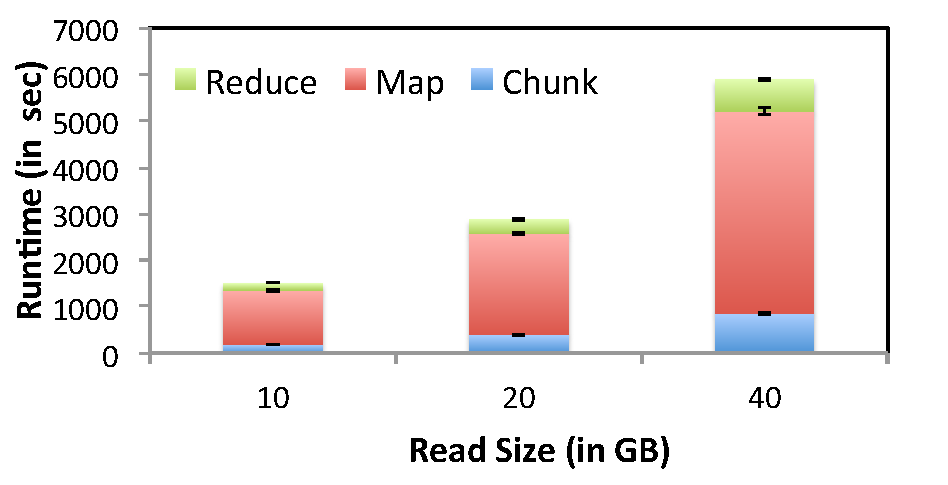
\includegraphics[scale=0.50]{figures/pj-smr-tts.pdf} 
\caption{\small Scale-out: Read size dependent time-to-solution for MapReduce task of read alignment and duplicate removal.  The number of nodes for this experiment,$N_W$ is 16, and the chunk size is set to contain 62500 reads.  The number of reducers is set to 8}
  \label{fig:read-size} 
\end{figure}

 In Fig.~\ref{fig:read-size}, the required scalability is measured with the increase of input data size.  It is apparent that compared to the map phase that conducts parallel alignment with BWA, other two steps, the reduce phase and the preparation of input data with multiple files are negligible.  Note that the alignment and the duplicate removal tasks are low-aggregation problems for MapReduce framework.  

Meanwhile, Fig~\ref{fig:scale-p-saga-mr} shows the overall good scaling results for the task of mapping and duplicate removal with PMR as the number of nodes used increases, indicating that PMR is a viable framework for delivering the good parallel performance against sizable data sets.





\begin{figure}
 \centering
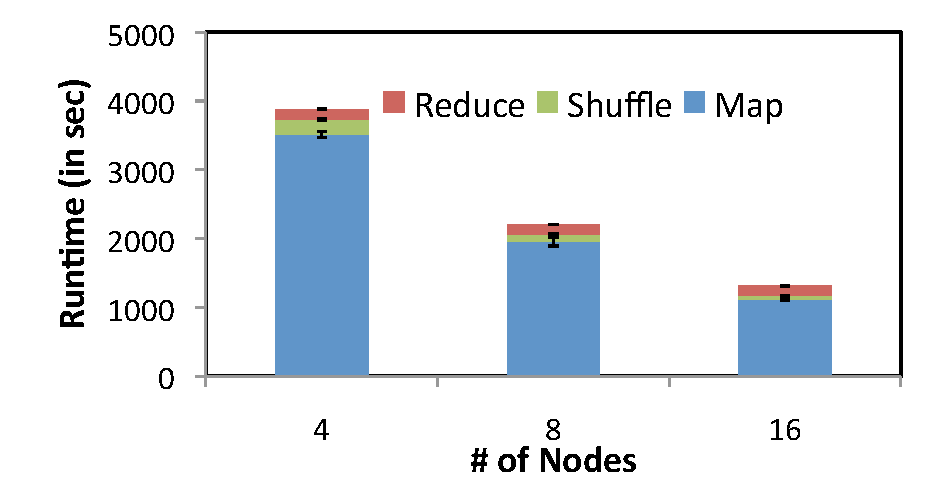
\includegraphics[scale=0.50]{figures/pj-smr-scale.pdf}
\caption{\small Scale-up: PMR scalability with read alignment and duplicate removal.  The number of works per node, $N_{W-n}$ is set to 2.   The input read is 10GB, the number of reducers is set to 8, The number of reads in a chunk is 625000.}
  \label{fig:scale-p-saga-mr} 
\end{figure}


\subsection{Comparison to Hadoop-based SEQAL and Crossbow}
\subsubsection{Closely Related Works}
There exist a few works specifically targeting NGS data analytics using the MR framework and four other tools are presented in Table~\ref{table:mr-comparison}.  In brief, Cloudburst was one of early tools to demonstrate the significant potential of MapReduce for NGS data analysis, whereas Crossbow focused on better scalability using Hadoop streaming.  Compared to the two Hadoop-based tools, GATK was introduced to support the general parallel execution pattern across many NGS data analytics.  Recently, the SEAL package was announced in which SEQAL is a utility for the alignment and duplicate removal.   

In spite of the commonality that MapReduce is the core programming model for the tools, they differ in several aspects depending upon the need of Hadoop, the way to utilize Hadoop, the level of flexibility for the extension of tools for alternative tasks or external tools such as aligners, and multiple cluster support.

Interestingly, multi-domain support with the MR framework is recently demonstrated for AutodDock application which is, in contrast to our applications that are loosely-coupled, pleasingly parallel.\cite{ecmls11-mr-autodock}

\begin{figure}
 \centering
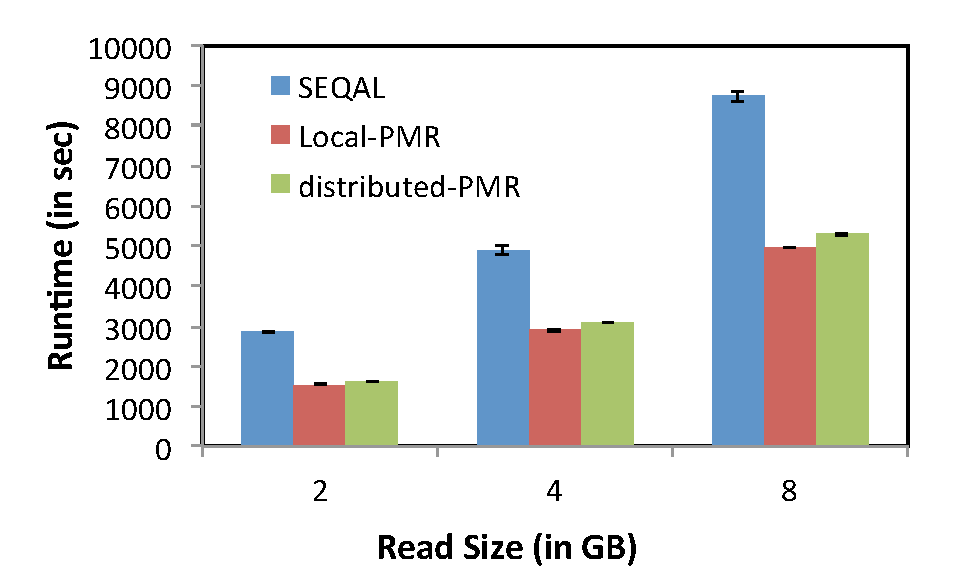
\includegraphics[scale=0.50]{figures/seqalvslocalpmr.pdf}

\caption{\small The total time-to-solution for MapReduce task of alignment and duplicate read removal.  Hadoop-based SEQAL is compared to Local-PMR vs. distributed-PMR.  BWA is the aligner for the map phase.  The size of input is 8 GB.  For this experiment, the number of nodes is 4, the number of workers (also Mappers) is 8, the number of Reducers is 8, and the number of reads in each chunk is 292,763. For the distributed-PMR, two machines of FutureGrid, Sierra and Hotel were used, whereas Sierra was used for other cases.}

  \label{fig:comp_with_seqal_1} 
\end{figure}

\subsubsection{Performance Comparison}
In Fig.~\ref{fig:comp_with_seqal_1} and Fig.~\ref{fig:comp_with_seqal_2}, we compared directly the time-to-solution between SEQAL and two scenarios with PMR, one with a single cluster and the other with two clusters.  In Fig.~\ref{fig:comp_with_seqal_2}, we dissect the contributions of each step for the total runtime.  

Notably, SEQAL takes more time on the overall run time, and the most contributing cause come from the map phase.  We interpret this result with the fact that the tmp directory on each node is used to store data by hadoop, but when the size of a tmp directory is limited for the required task, a remote file system is configured as  the tmp data directory for remote disks of other nodes.

Another observation from Fig.~\ref{fig:comp_with_seqal_1} and Fig.~\ref{fig:comp_with_seqal_2} is that whereas SEQAL is limited by a single cluster with Hadoop, PMR can be easily scale-across multiple clusters. The distributed-PMR is indeed performing well against local-PMR without significant performance loss due to the low connectivity between two clusters with our experimental set up.  

Again, Fig.~\ref{fig:comp_with_seqal_2} clearly indicates the map phase for SEQAL has a disadvantage against PMR.  The comparison of the reduce phase could originate from the different implementation between SEQAL and ours.

\begin{figure} 
 \centering
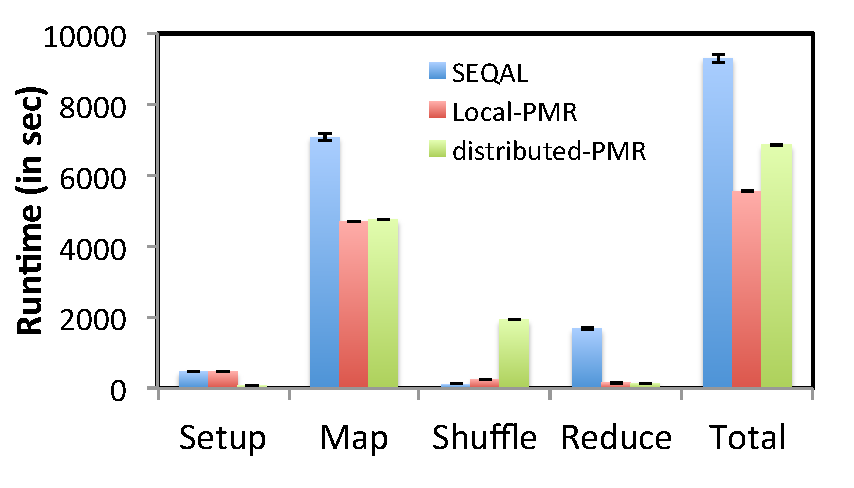
\includegraphics[scale=0.50]{figures/8GB_phasewisetimes.pdf}
\caption{\small  Dissected elapsed times for each step in the results shown in Fig.~\ref{fig:comp_with_seqal_1}.  }
  \label{fig:comp_with_seqal_2} 
\end{figure}


\begin{figure} 
 \centering
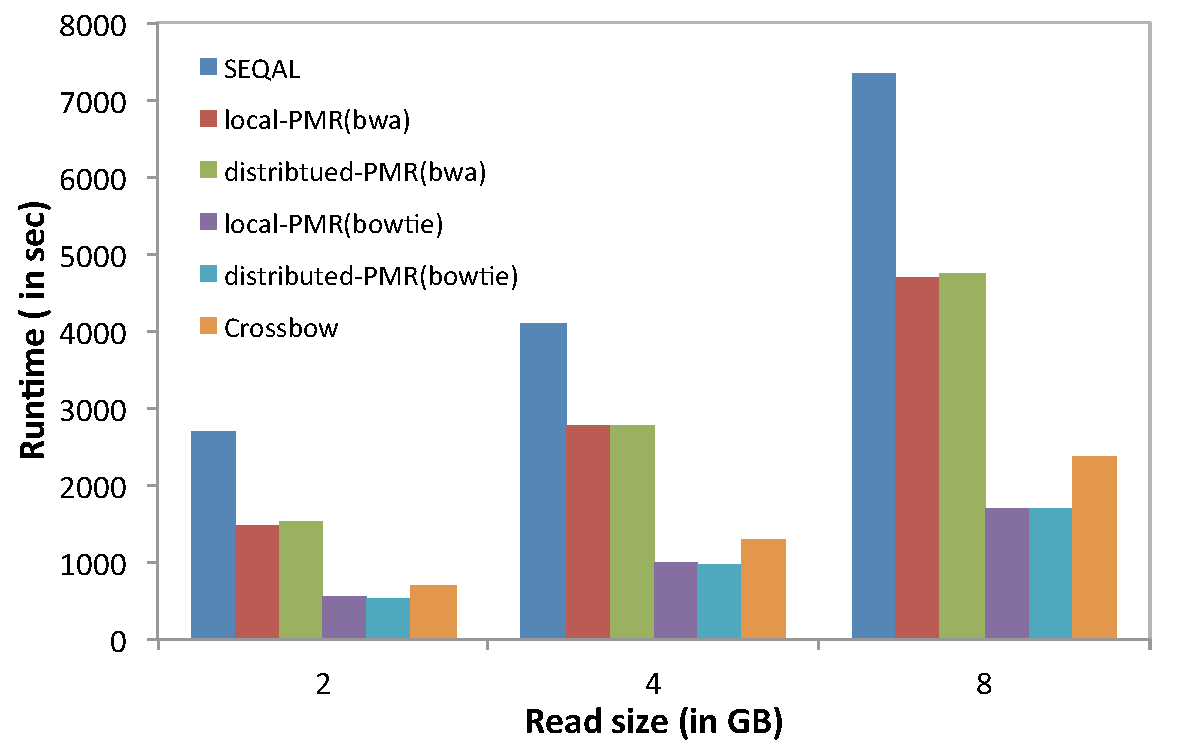
\includegraphics[scale=0.40]{figures/map_comp.pdf}
\caption{\small  Map phase comparison.  The runtimes for the Map phase of SEQAL, Local-PMR(BWA), distributed-PMR(BWA), Local-PMR(Bowtie), distributed-PMR(Bowtie), and Crossbow(Bowtie) are compared.  The aligner used for each case is indicated in a parenthesis.  For this experiment, the number of nodes is 4, the number of workers is 8, and the number of reads in each chunk is 292,763.  For the distributed-PMR, two machines of FutureGrid, Sierra and Hotel were used, whereas Sierra was used for other cases.}
  \label{fig:tool_comp} 
\end{figure}

%number of nodes=4, number of workers/node=2,reduces=8, number of reads/chunk=292763; ********DMR provides scale-across********** as two machines sierra and hotel are used.



As the number of input sequences increased the time to solution also increased linearly for both SEQAL and local-PMR. 
The time to solution decreased by an average of 43.39\% with 95\% confidence interval of 3.03\%. The Map phase of Local-PMR is on an average of 64\% of Map phase of SEQAL application, and is reduced by an average of 35.7\%
The reduce phase is very less compared to seqal applicaiton because there is not sort involved in reduce phase.
\pmnote{( why is that?? i dont see any reason to have a sort before reduce starts)) we do sort intermediate data before shuffled.}
The reduce phase is average of 8.85\% of reduce phase of seqal  ( it involves sort )

\pmnote{how to explain performance of PMR ??}..One of the performance bottlneck for PMR is coordination system used... we used redis as coordination system... which is proved best ,when compared to other coordination systems{Pstar reference}. I think we can compare the results.. but cant say why SEQAL performed better.. since, it needs understanding of how SEQAL actually works.


\section{Discussions and Concluding Remarks}\label{sec:discussions}
\subsubsection{PMR vs. Existing other approaches}

On the other hand, in spite of many advantages including fault-resilency and easy scalability within a cluster, Hadoop-based approaches such as Crossbow, Cloudburst, and SEAQL are also limited by the nature of Hadoop.  Firstly, the overall performance of Hadoop-based MapReduce is determined by the unknown network performance and the connectivity between the data storage and the compute which are determined by characteristics of the cluster Hadoop is installed.  The tight coupling between the MapReduce applications with underlying Hadoop causes unnecessary complexity when the optimization or the design of parallel execution is required.  Secondly, it is not trivial to scale across different clusters.  Many issues on the connectivity between two separate clusters including firewalls, different security policies, and potentially different administration structure are making difficult to extend Hadoop with other cluster systems.  Thirdly, it is a still ongoing concern that Hadoop's current implementation has obstacles from the scalability issue with the design with Namenode and Job tracker.   The open source Hadoop is implemented with a job and task tracker: the job tracker is the central manager that dispatches map and reduce tasks to the nodes(nodes could be from multiple clusters) of the Hadoop cluster. On each node the task tracker is responsible for executing the respective tasks. The main limitation of this architecture is the fact that it intermixes both cluster resource management and application-level task managements. Thus, it is e.g. not easily possible to integrate Hadoop with another resource management tool, e.g. PBS or Torque. Also, the job tracker represents a single point of failure and scalability bottleneck. Another limitation is the latencies between machines should not be so big as HDFS uses Avro - an RPC-style protocol for communications.

Collectively, PMR has edges in terms of flexibility and non-Hadoop-based architecture

\subsubsection{PMR, a viable solution for scale-across and extensible framework for NGS data analytics}


\subsubsection{DARE and beyond}
PMR-based NGS tools, implemented and scrutinized in this work, were developed in conjunction with our development of the runtime environment for dynamic applications, Dynamic Application Runtime Environment (DARE).  DARE is our strategically important component for the development of Science Gateway for NGS data analytics and downstream analysis.  Under the design strategy of DARE-based gateways, PMR-based tools were conceived to be a category of supporting execution patterns for parallel and distributed task and data management.  




\section*{Acknowledgement}
This document was developed with support from the National Science
Foundation (NSF) under Grant No.  0910812 to Indiana University for
``FutureGrid: An Experimental, High-Performance Grid Test-bed.''  We
also acknowledge the SEAL developer, Luca Pireddu for useful performance related
discussions, and Erik Flemington for allowing us to use his RNA-seq data sets. Computing resources were made possible via NSF TRAC award TG-MCB090174 and LONI resources.  The project described was partially
supported by Grant Number P20RR016456 from the NIH National Center For
Research Resources.

\bibliographystyle{abbrv} 
\bibliography{compbio,saga}


\end{document}

Any opinions, ndings, and conclusions or recommendations expressed in
this material are those of the author(s) and do not necessarily
reflect the views.
